\documentclass[conference]{IEEEtran}
% *** CITATION PACKAGES ***
%\usepackage{cite}
% *** GRAPHICS RELATED PACKAGES ***
\ifCLASSINFOpdf
   \usepackage[pdftex]{graphicx}
\else
  \usepackage[dvips]{graphicx}
  \usepackage{epsfig}
\fi
\usepackage{threeparttable}
%\usepackage[cmex10]{amsmath}
\usepackage{amsmath}
\usepackage{arydshln}
\usepackage[numbers,sort&compress]{natbib}
\usepackage{float}
\usepackage{dblfloatfix}

\begin{document}

\title{Phasen, Techniken und Strategien der Softwareentwicklung anhand eines Kursprojekts im Modul SWE-II}

\DeclareRobustCommand{\IEEEauthorrefmark}[1]{\smash{\textsuperscript{\footnotesize #1}}}

\author{\IEEEauthorblockN{Felix Jacobsen\IEEEauthorrefmark{1},
Dennis Podkolsin\IEEEauthorrefmark{2} und Marcus Koppelmann\IEEEauthorrefmark{3}}
\IEEEauthorblockA{Fachbereich Duales Studium, Studiengang Informatik\\ 
Hochschule für Wirtschaft und Recht Berlin\\
Email: \IEEEauthorrefmark{1}s\_jacobsen20@stud.hwr-berlin.de,
\IEEEauthorrefmark{2}s\_podkolsin20@stud.hwr-berlin.de,
\IEEEauthorrefmark{3}s\_koppelmann20@stud.hwr-berlin.de}}

\maketitle

% --- Abstract ---
\begin{abstract}
\boldmath
Der geschlechterbewusste und inklusive Sprachgebrauch findet insbesondere im pädagogischen, wie auch im akademischen und medialen Bereich immer mehr Verwendung. So werden unter anderem wissenschaftliche Arbeiten von Student*innen sowie journalistische Artikel und Recherchen in genderneutraler Sprache verfasst. Das Schreiben dieser genderneutralen Texte kann eine zusätzliche Herausforderung für die Autor*innen bedeuten. Unterschiedliche Schreibstile bedürfen individueller Eingewöhnungszeiten. Um dieses Problem anzugehen, schlagen wir im vorliegenden Paper im Rahmen des Kursprojekts des Moduls Software Engineering II (SWE-II) der HWR Berlin eine neuartige Softwarelösung vor, welche Text in eine genderneutrale Form bringt. Unser Ansatz zielt darauf ab, eine zielgruppengerechte, durch Endanwender*innen nutzbare Möglichkeit für das automatisierte Gendern von Texten zu bieten. Basierend auf gängigen Regeln des Genderns in deutscher und in englischer Sprache werden hierfür die technischen Möglichkeiten des \textbf{Natural Language Processing (NLP)} betrachtet. Die zugehörigen Phasen der Softwareentwicklung und die Arbeitsweise mit der Planung, der Erarbeitung der Softwarearchitektur, der Implementierung und der Qualitätssicherung werden im Kontext des Moduls SWE-II beschrieben.
\end{abstract}

% --- Stichwörter ---
\begin{keywords} 
Softwareentwicklung, Gendern, Natural Language Processing, Textverarbeitung
\end{keywords}

% --- Einleitung/Forschungsfrage ---
\section{Einleitung}
\label{sec:einleitung}
% Dennis

% Erklären Sie hier gerne, warum Sie das Projekt machen, warum es wichtig ist und wo die Motivation her kommt. Eine Forschungsfrage könnte sich unter anderem daraus ergeben, wenn Sie fragen, wie Sie das Projekt umsetzen können. Also sowas ähnliches wie "Wie kann das Projekt XYZ unter Berücksichtigung des Softwarelebenszykluses erfolgreich implementiert werden?"


%Die vorliegende wissenschaftliche Ausarbeitung beschreibt den Entwurfs- und Entwicklungsprozess der Assistenzwebanwendung "Equaly", als des Moduls „Software Engineering II“.

%Dabei handelt es sich um die Weiterführung des Softwareprojekts „Genderly“ des vorhergehenden Moduls „Software Engineering I“.\\
%„Genderly“ sowohl als auch „Equaly“ dienen dem Nutzer als Hilfe bei der Verfassung von Texten, indem sie dem Nutzer das Einhalten von Gendernormen erleichtern.
%Um Dies zu erreichen, wird der Text analysiert und anschließend wird dem Nutzer ein bearbeiteter Text, in Form eines Gendervorschlages, präsentiert. 
%Der generierte Gendervorschlag basiert auch verschiedenen Faktoren, unteranderem auch dem Genderstil. Während der Entwicklung wurden verschiedene Genderstile festgelegt und sogenannte „Nice to Haves“ und „Must Haves“ aufgeteilt. Während Aufteilung dieser „Nice to Haves“ und „Must Haves“ wurde entschieden, dass der primäre Genderstil der „Wortersatz“ sein wird.
%Diese Fähigkeit des Wortersatzes wurde zur Kernfunktion unserer Anwendung und mit Hilfe einer Datenbank und KI Pipeline realisiert.
%Die Entwicklungs- und Dokumentationsphasen, die zur Finalisierung des Softwareprojektes „Equaly“ geführt haben, werden in der folgenden Ausarbeitung thematisiert und dargestellt.  

% Wie wird an der HWR Berlin Software Engineering vermittelt.
% (Paper von Frau Monett Díaz zitieren, wenn über Struktur und Aufbau des Unterrichts kurz geredet wird)
% "im 3. Semester das und das gemacht, im 4. Semester das und das ..."
% "Im Rahmen dieses Moduls ... Entwicklungsprinzipien lernen und praktisch anwenden"
% "Aufgabe: Eine Software für eines der 17 Ziele der UN entwickeln, durch alle Phasen des Softwareengineerings führen"
% "Dabei auch Qualitätssicherung und Einholen von Feedback praktiziert"


Das Verfassen von Texten verschiedenster Art, unabhängig von ihrem Inhalt, hat immer das Ziel, möglichst viele Leser*innen der gewählten oder auch weiterer Zielgruppen anzusprechen. Dies kann auf verschiedenste Art und Weise erreicht werden, z.B. durch bestimmte Stilmittel. Das Einbinden aller Geschlechter (Gender) in die Zielgruppenfindung und die Sprache stellt dabei einen der effektivsten Wege dar, eine breite Leserschaft zu adressieren.

Um dies zuverlässig zu erreichen, wird von den Autor*innen erwartet, ihre Texte in grundlegenden Aspekten an die Erwartungen der Leserschaft anzupassen. Der Anpassungsprozess durch z.B. Umformulierungen kann dabei viel Zeit und Energie der Autor*innen in Anspruch nehmen. Diese Änderungen und ihr Aufwand treten nicht nur während des Verfassens, sondern u.U. auch nach der inhaltlichen Fertigstellung eines Werkes auf. Das kann der Fall sein, wenn sich die von der Gesellschaft und der gewünschten Leserschaft erwarteten Gendernormen im Nachhinein verändern.

Genau an dieser Stelle besteht der Bedarf für Equaly. Mit Hilfe von automatischer Texterkennung und Textanalyse ist es in der Lage, genderspezifische Ausdrücke mit genderneutralen Begriffen auszutauschen. 

Equaly ist das Ergebnis einer Gruppenarbeit im Rahmen der Module  ''Software Engineering I'' und ''Software Engineering II'' des Informatik Fachbereichs der Hochschule für Wirtschaft und Recht Berlin.
Diese Module fanden während des 3. und 4. Semesters des Studiums statt. Die Module hatten das Ziel, im Laufe eines Semesters und begleitend zu den Vorlesungen und Laboren den Studierenden zu ermöglichen, ihr eigenes Softwareprojekt zu planen, zu dokumentieren und eine Softwarelösung zu entwickeln.
Dabei wurde gelehrt, diverse Entwicklungsprinzipien praktisch anzuwenden.

Die im Modul gegebene Aufgabenstellung für das Softwareprojekt war es, eine Software für eines der 17 Ziele der UN zu entwickeln. Dabei galt es, alle Phasen des Software-Engineerings zu durchlaufen. Innerhalb des Entwicklungsprozesses wurden so auch Qualitätssicherungspraktiken durchgeführt und das Feedback von Testpersonen im Rahmen eines Beta-Tests eingeholt.
% --- Ausgangslage/ Erklärung SWE II ---
\section{Ausgangslage}
\label{sec:ausgangslage}
% Dennis

% Weniger KI, mehr SWE II
% Du beschreibst hier schon die Systemarchitektur

% Erst alles historische (und hysterische) zu Genderly
% Dann "Brücke" zu Weiterentwicklung Equaly
% Dann sagen, warum Weiterentwicklung (weil eben so in Semester 4 erwartet und weil Verbesserungsvorschläge erarbeitet wurden)

Equaly ist eine Weiterführung des Softwareprojekts Genderly des Vorgängermoduls ''Software Engineering I'' aus dem dritten Semester. Genderly dient dadurch als Grundlage für die Weiterentwicklung unter dem neuen Namen Equaly.

Genderly hatte das gleiche allgemeine Ziel wie das jetzige Equaly, jedoch wurde in der Entwicklung ein anderer Ansatz verfolgt als in Equaly. Das Ziel von dem Modul ''Software Engineering I'' war, einen funktionsfähigen Prototyp zu erarbeiten. Im Vorfeld ist es jedoch nötig gewesen, sich in die Thematik der Verarbeitung natürlicher Sprachen einzuarbeiten. Das Ergebnis dieser Arbeit war eine auf Java basierende Webanwendung mit HTML5-Frontend und rudimentärer Datenbank. In deutschen Sätzen wurden Worte mit Großbuchstaben herausgefiltert und gegen die Einträge dieser Datenbank geprüft. Sofern hier ein genderneutrales Ersatzwort gefunden wurde, wurden Vorgänger und Nachfolger des Wortes darauf geprüft, ob sie Artikel sind. War das der Fall, wurden auch sie an das neue Substantiv angepasst.

Die Anforderung des Nachfolgemoduls ''Software Engineering II'' bestand nun daraus, die Weiterentwicklung dieses Softwareprojektes zu einer ausgereifteren Softwarelösung durchzuführen.
% --- Genderneutrale Sprache (das Problem im Kern betrachtet) ---
\section{Genderneutrale Sprache}
\label{sec:sprache}
% Dennis

Sprache ist allgegenwärtig und dient nicht immer nur als Kommunikationsmittel. 
Sie kann informieren, aber auch unterhalten. Parallel dazu wandelt sie sich so beständig, wie die Gesellschaft. Dies ist unter anderem auch im Gebiet des Genderns zu beobachten. Gendern wird zusehens Teil der alltäglichen Sprachpraxis. Gendergerechte Sprache ist ein weiterer Schritt im immer andauernden Entwicklungsprozess der Sprache und Sprachpraxis. Sie stellt eine Möglichkeit dar, Informationen durch eine diversere Sprachvielfalt inklusiver zu gestalten und stellt damit einen Beitrag zur Gleichberechtigung dar.

Diese ursprüngliche, dominant männliche Sprachorientierung wird mit Hilfe des generischen Maskulinums realisiert. Wenn das generische Maskulinum genutzt wird, werden allgemeine Personengruppen mit der männlichen Form dargestellt. Dabei wird zum Beispiel eine Gruppe aus Studierenden als ``Studenten'' bezeichnet. Ohne dabei zu berücksichtigen, dass sich in der Gruppe möglicherweise weibliche Studenten -sprich Studentinnen- befinden können. Dies ist eine weit verbreitete, da historisch gewachsene sprachliche Konvention \cite{Hei00}.

Diversifikation der Sprache findet sowohl verbal, als auch schriftlich statt. In textueller Form wird dies durch die richtigen Sprachmittel erreicht. Eine Möglichkeit, Genderneutralität in einem Text zu erreichen, ist die genderneutrale Sprache durch Einhaltung von Gendernormen. Diese Gendernormen können wiederum unterschiedliche Regelsätze zur Wortbildung bzw. Umformulierung bedeuten.

Einer dieser Regelsätze wird zum Beispiel mit der Verwendung des Gendersterns angewendet. Bei dieser Schreibweise wird versucht, das männliche und das weibliche Geschlecht in gemeinsamen Ausdrücken zu vereinen. Beispielsweise wird dadurch eine Gruppe von Studierenden nicht mehr als Studenten, sondern als ``Student*innen'' bezeichnet. Der Genderstern agiert hierbei als Verbindungssymbol zwischen dem generischen Maskulinum und der Wortendung ``-in/-innen''. Alternativ lässt sich der Genderstern auch durch andere Symbole, wie zum Beispiel den Doppelpunkt, das Semikolon oder auch den Schrägstrich ersetzen. Diese Alternativen bilden Beispiele von Genderstilen der Schrift. Ein Genderstil, der bei einer Untermenge genderbarer Wörter angewendet werden kann, ist der vollständige Wortersatz. Dadurch kann eine bessere Lesbarkeit eines Textes gewährleistet werden. Jedoch fordert dieser Genderstil die meiste Aufmerksamkeit des Autors.

Bei der Nutzung des Genderstils des vollständigen Wortersatzes werden genderspezifische Begriffe durch genderneutrale Alternativbegriffe ersetzt. So wird beispielsweise eine Gruppe von ``Männern'' als eine Gruppe von ``Personen'' bezeichnet. Der Vorteil dieses Genderstils ist, dass der Lesefluss eines Textes, anders als bei der Nutzung des Gendersterns, nicht beeinträchtigt wird. Die Beeinflussung des Leseflusses wird beim lauten Vorlesen eines Textes besonders deutlich, da das Aussprechen des Gendersterns beispielsweise keine konkrete Vorgabe in der deutschen Sprache hat. Ein weiterer Nachteil des Gendersterns, den der Wortersatz nicht besitzt, ist, dass einige Wörter nicht gegendert werden können. Beispielsweise kann die Bezeichnung ``Mann'' nicht zu ``Mann*in'' umgeformt werden. Mit Hilfe des Stils des Wortersatzes ist Gendering hier hingegen möglich.
% --- Arbeitsweise (wie wir uns für die Projektarbeit organisiert haben) ---
\section{Arbeitsweise}
\label{sec:arbeitsweise}
% Felix

Equaly ist ein Softwareprojekt und benötigt zwecks seiner Weiterentwicklung eine Projektorganisation. Dadurch wird die Arbeit innerhalb des Projektteams strukturiert und im Ablauf optimiert. Beim vorliegend betrachteten Softwareprojekt ist das gesamte Team für die Organisation verantwortlich. Das Team arbeitet grundsätzlich zusammen. Bei den zu erledigenden Aufgaben bringt sich jedes Teammitglied mit ein. Für die Kommunikation innerhalb des Teams wurde eine Discord-Gruppe erstellt. Das Team kommuniziert hier regelmäßig zu wöchentlichen Standups, diskutiert über die noch zu erledigenden Aufgaben und plant hier das weitere Vorgehen.

Des Weiteren wurde für das Softwareprojekt eine GitHub-Organisation\footnote{Link zur GitHub-Organisation: \href{https://github.com/HWR-Berlin-SWE-II-Gruppe-2-Team-3-2022}} mit je einem Dokumentations- und einem Software Repository gegründet. Durch die Nutzung von GitHub kann das Team gemeinsam an der Software arbeiten, den geschriebenen Code strukturiert verwalten und überprüfen. Hinzu kommt, dass eine automatische Versionierung mittels Git von Beginn an sichergestellt wird. Die Repositories sind jeweils öffentlich einsehbar, um den Entwicklungsprozess im Rahmen des Moduls nachvollziehbar und transparent zu gestalten.

Eine klar abgegrenzte Rollenverteilung ist bewusst nicht vorhanden. Jedoch hat jedes Teammitglied ein Spezialgebiet, sodass je nach Aufgabe ein Mitglied das Grundgerüst erstellt, welches vom Rest des Teams durch Anmerkungen und Reviews ausgearbeitet und verfeinert wird. Dennis ist so für das Testing, die Test Infrastruktur und das Mocking zuständig. Felix erarbeitet in Abstimmung die Dokumentation, das Wording und das Marketing. Marcus ist für die Entwicklung zuständig.
% --- Zielgruppenanalyse (Wer ist warum in welcher Form in der konkreten Projektumsetzung als Nutzer mit seinen Bedürfnissen berücksichtigt?) ---
\section{Zielgruppenanalyse}
\label{sec:zielgruppenanalyse}
% Felix

Bei der Entwicklung von Applikationen muss darauf geachtet werden, für welche Zielgruppen die Anwendung entwickelt wird. Die Zielgruppen sollen die zukünftigen Anwender*innen der Software sein. Sie bilden einen wesentlichen Teil der Stakeholder*innen.

Da im akademischen Raum das Gendern umfassend an Bedeutung gewinnt, ist entsprechend davon auszugehen, dass es sich bei den zukünftigen Anwender*innen zu einem großen Anteil um Studierende handeln wird. Deshalb orientiert sich die Anwendung insbesondere an dieser speziellen Zielgruppe. Die Applikation soll die Studierenden beim einfachen und korrekten Gendern in wissenschaftlichen Texten unterstützen. Für Student*innen ist es wichtig, dass sie einen geringen Arbeitsaufwand bei der Nutzung der Software erfahren. Insofern muss die Anwendung einfach benutzbar sein.

Die Software kann auch von Dozent*innen genutzt werden. Die Verwendung der Applikation findet in diesem Fall vorwiegend im didaktischen und pädagogischen Zusammenhang statt. Die Dozent*innen beabsichtigen dabei, ihren Lehrauftrag zu erfüllen, welcher indirekt auch die Vermittlung der Gleichberechtigung der Geschlechter beinhaltet. Dafür muss die Software einfache, flexible und mobile Anwendungsmöglichkeiten bereitstellen.

Eine weitere Zielgruppe sind Lehrkräfte \& Schüler*innen. Die Lehrkräfte haben wie die Dozent*innen ein ausgeprägtes Interesse an der einfachen und flexiblen Anwendung des Produkts. Sie verfolgen ebenso das Ziel, ihren Lehrauftrag zu erfüllen, welcher die Vermittlung der Gleichberechtigung der Geschlechter beinhaltet. Schüler*innen möchten gleichzeitig die eigentlichen Textinhalte sehr leicht lernen können. Beide Gruppen nutzen die Software als Hilfsmittel während des Schreibens. Besonders zu betonen ist hierbei das potenzielle Alter der Anwender*innen. Sowohl sehr junge, als auch sehr erfahrene Menschen sollen die Software nutzen können. Equaly soll die Nutzer*innen bei der Erweiterung ihres Wissens über genderneutrales Schreiben unterstützen. Wegen der großen Altersspanne ist eine stark vereinfachte Bedienung erforderlich.

Weitere mögliche Anwender*innen der Software sind Politiker*innen und Journalist*innen. In Teilen der Politik und des Journalismus wird vermehrt Wert auf inklusives Schreiben gelegt. Das Ziel dabei ist es, dass sich dass Publikum besser angesprochen und stärker einbezogen fühlt, damit die Politiker*innen oder Journalist*innen eine möglichst große Wählerschaft beziehungsweise eine möglichst große Leserschaft erreichen. Diese Zielgruppe hat jedoch keinen großen Einfluss auf die Anforderungen der Applikation, deswegen wird sie in diesem Absatz nur kurz erwähnt, im folgenden Text aber nicht weiter auf sie eingegangen.
% --- Gesamtarchitektur (hier kommt dann ein „allumfassendes“ UML rein) ---
\begin{figure*}[!t]
    \centering
    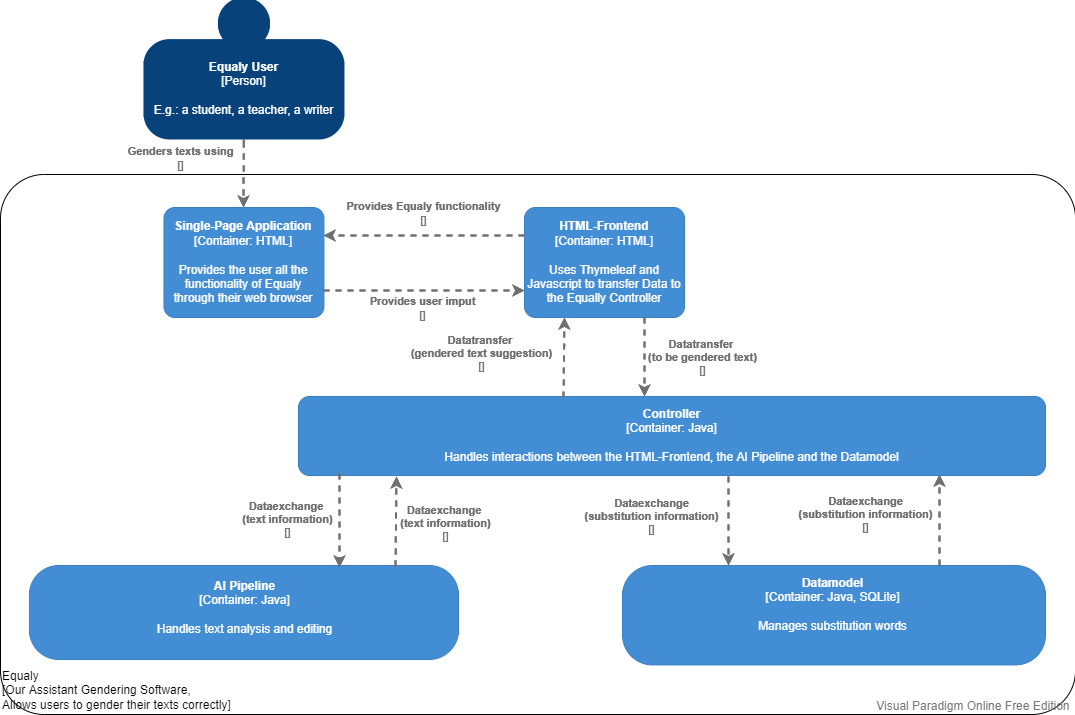
\includegraphics[width=13cm]{Resources/C2.png}
    \caption{C2-Softwarearchitektur von Equaly}
    \label{fig:c2}
\end{figure*}
\section{Softwarearchitektur}
\label{sec:softwarearchitektur}
% Marcus

Basierend auf der erstellten Zielgruppenanalyse gilt es, die Architektur der zu entwickelnden Software zu entwerfen. Diese stellt für das System die fundamentale Organisation durch Komponenten, ihre Beziehungen und ihre Umwelt dar \cite{Hi00}. Die resultierende Architekturbeschreibung dient zusätzlich als Dokumentation und als wesentliche Kommunikationsgrundlage für die Stakeholder*innen des Projekts.

Mit dem strategischen Entwurf der Architektur wird insbesondere berücksichtigt, dass Vertreter der ausgemachten Zielgruppen die Software optimal erreichen, nutzen und unkompliziert von ihrer Funktionalität profitieren können. Bei den ermittelten Zielgruppen ist jeweils eine hohe Variation verwendeter Endgeräte festzustellen. Mit unterschiedlichen Endgeräten werden wiederum sehr unterschiedliche Arbeitsaufgaben wahrgenommen. Das Verfassen journalistischer Artikel kann beispielsweise entsprechend in einer statischen Büroumgebung, aber auch mittels mobiler Endgeräte stattfinden. Eine ähnliche Vielfalt kann im akademischen Bereich für Schüler*innen, Dozent*innen und Student*innen bei der Erarbeitung von Texten, Berichten und wissenschaftlichen Ausfertigungen beobachtet werden.

Die Softwarearchitektur ist entsprechend derartig zu gestalten, dass eine schließlich realisierte Softwarelösung für eine größtmögliche Anzahl potenzieller Nutzer*innen verwendbar ist. Gleichzeitig soll sie für eine Vielzahl von Endgeräten einheitliche Funktionalität bieten, da andernfalls der Entwicklungsaufwand das Zeitbudget des Kurses übersteigen würde. Basierend darauf wurde entschieden, Equaly als Web-Applikation zu entwickeln. Unterschiedliche Geräte können dadurch mit niedrigem lokalen Ressourcenbedarf Ergebnisse anzeigen, da die Geschäftslogik mit dieser Art der Software auf einen Webserver ausgelagert werden kann. Die Faktoren der Zuverlässigkeit und der Anpassbarkeit von Equaly werden dadurch zentral für das Entwicklerteam adressierbar. Der Zugriff auf Web-Applikationen erfolgt parallel durch mehrere Nutzer mittels Webbrowser, welcher statt einer eigenen, spezialisierten Client-Software die Rolle des Thin-Client einnimmt \cite{Wu01}.

Mit Festlegung der Anwendungsart muss die Frage nach den zu verwendenden Technologien beantwortet werden.
Aufgrund von Vorwissen und Erfahrung innerhalb des Teams wird für das Backend der Web-Applikation Java unter Verwendeung des Spring-Frameworks genutzt. Für das Frontend werden HTML, CSS, JavaScript und Thymeleaf verwendet. Letzteres dient als Übertragung der Informationen zwischen Frontend und Backend.

Die geplante Kernkompetenz der Anwendung, die Sprachverarbeitung, muss beim Aufbau der Architektur in seiner Komplexität berücksichtigt werden. Mit Feedback zum bereits eingereichten Prototyp konnte festgestellt werden, dass für die Sprachverarbeitung ein deutlicher Bedarf für den Einsatz von künstlicher Intelligenz besteht. Aufgrund von vorhergehenden Erfahrungen im Team findet das vorab trainierte KI-Modell der Bibliothek Lingua für die Sprachermittlung Verwendung. Mehrere ebenfalls vortrainierte KI-Modelle aus der Bibliothek OpenNLP realisieren dann Textanalysen und Klassifikationen. Zur geplanten Realisierung eines Dictionaries wird eine SQLite-Datenbank genutzt. Hier sollen genderbare Wörter und ihre jeweiligen Alternativen eingetragen und verfügbar sein, wie auch in \ref{fig:c2} mit der C2-Architekturdarstellung gezeigt ist.
Als Architekturmuster wird, aufgrund der bis hierhin klar unterteilbaren Softwarekomponenten, das Architekturmuster Model-View-Controller (MVC) genutzt.
% --- Theoretische Betrachtung des Designs (Wie wollen die Nutzer das? Bedienoberfläche: Design, Ergonomie)
\section{Entwurf der Bedienoberfläche}
\label{sec:substitution}
%Marcus

Im Rahmen der Kursarbeit gilt es, die Entwurfsgrundsätze von Bedienoberflächen kennenzulernen, auf das eigene Softwareprojekt anzuwenden und eine Auswahl aus unterschiedlichen Möglichkeiten zur Informationsdarstellung basierend auf Vor- und Nachteilen zu treffen. Dazu wird der Vorgang des Oberflächenentwurfs als iterativer Prozess aufgefasst, in welchem das Team als Designer und Entwickler die Zielgruppenanalyse als Handlungsbasis für den Entwurf von Mockups interpretiert. Dadurch bilden die Entwürfe der Bedienoberfläche ein direktes Resultat der Beobachtung der Benutzer, ihrer Aufaben und Intentionen \cite{La05}. Für Equaly bedeutete dies den Entwurf einer Weboberfläche für Texteingabe und Anzeige des gegenderten Textresultats. Die Diversität der ausgemachten Zielgruppen und die geplante Platzierung von Equaly als Hilfsmittel führten zu dem Entschluss, die Oberfläche möglichst übersichtlich und einfach aufzubauen. Für den Gendering-Prozess bildet der nutzerseitig eingegebene Text die Handlungsgrundlage. Entsprechend sollte die Oberfläche um die Kernkompetenz der intuitiven Ein- und Ausgabe von Text aufgebaut werden. Der aus dieser Phase favorisierte Mockup ist in \ref{fig:mockup} dargestellt.

\begin{figure}[!th]
\centering
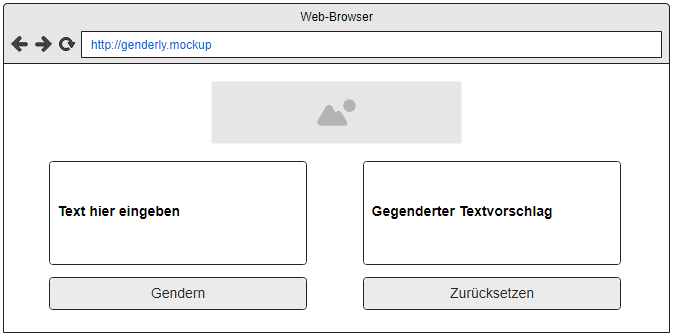
\includegraphics[width=8cm]{Resources/Mockup.PNG}
\caption{Favorisierter Mockup für die Weboberfläche von Equaly}
\label{fig:mockup}
\end{figure}

Neben der Anordnung der Elemente wurde auch die farbliche Gestaltung entworfen. Es galt, Farben derartig einzusetzen, dass die Oberfläche einen Wiedererkennungswert und Aufmerksamkeit bei den Zielgruppen erreichen würde. Eine erarbeitete Farbgebung richtete sich danach, wie die UN für das 5. Ziel für die nachhaltige Entwicklung gestaltete. Die entsprechend orange Gestaltung sollte Aufmerksamkeit erregen, gleichzeitig aber auch die positive Motivation hinter Equaly unterstreichen.
% --- Substitution genderbarer Satzteile (Der „Kern“ des Ganzen, und nur der) ---
\section{Substitution genderbarer Textbestandteile}
\label{sec:substitution}
%Marcus

Als Kernfunktionalität der Software Equaly ist die Verarbeitung von eingegebenem Text zu gegendertem Text zu realisieren. Text muss dafür durch das Frontend aufgenommen und im Backend zumindest anteilig substituiert werden. Dazu wurde unter Verwendug der ausgewählten Technologien eine mit \ref{fig:pipeline} dargestellte KI-Pipeline entwickelt. Unverarbeiteter Text wird zunächst in seiner Gesamtheit an einen \textit{Language Detector} der Bibliothek Lingua\footnote{Die Bibliothek wurde über https://github.com/pemistahl/lingua bezogen.} weitergegeben. Dieser findet Verwendung, da er besonders wenig Text benötigt, um die verwendete Sprache bereits identifizieren zu können.

\begin{figure}[!th]
\centering
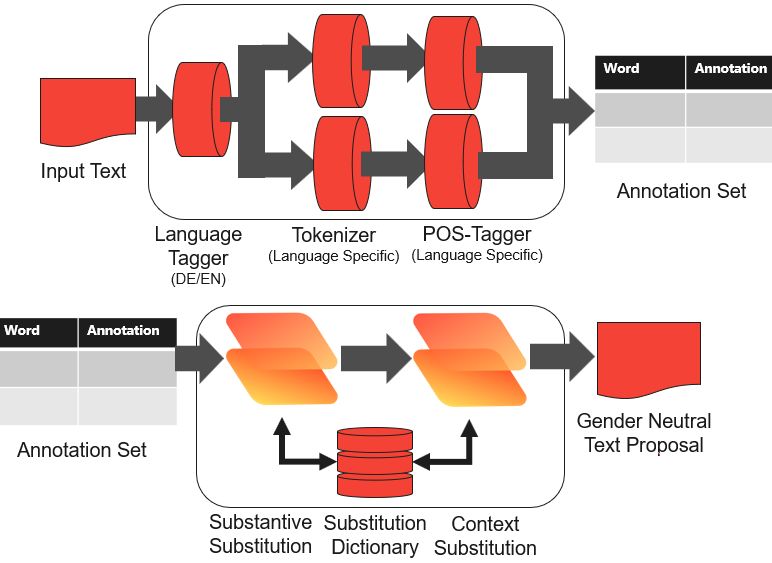
\includegraphics[width=9cm]{Resources/Pipeline.PNG}
\caption{Schematische Darstellung der KI-Pipeline}
\label{fig:pipeline}
\end{figure}

Abhängig von der erkannten Sprache, welche entweder Deutsch oder Englisch sein soll, wird anschließend ein Tokenizer-Modell der Bibliothek OpenNLP auf den Text angewendet. Die damit stattfindende Zerlegung in Sinnbausteine des Texts resultiert in einem Datensatz bestehend aus Token bzw. einzelnen Wortelementen. Diese Tokenmenge wird, erneut abhängig von der zuvor ermittelten Sprache, einem Part-of-Speech-Tagger (POS-Tagger) zugeführt. Der POS-Tagger wendet dabei ein vortrainiertes Maxent-Modell\footnote{Die verwendeten Modelle für Tokenizer und POS-Tagger wurden über http://opennlp.sourceforge.net/models-1.5/ bezogen.} an. Zwischenergebnis ist nun eine mit ihrer Sprache identifizierte Menge an Token, wobei die Token wie in \ref{fig:pos} zu sehen, durch den POS-Tagger mit Tags versehen wurden.

\begin{figure}[!th]
\centering
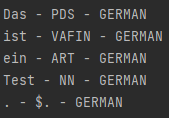
\includegraphics[width=2.5cm]{Resources/POS.PNG}
\caption{Ausgegebenes Zwischenergebnis der KI-Pipeline}
\label{fig:pos}
\end{figure}

Durch die angefügten Tags werden z.B. Substantive, irreflexible Personalpronomen und Eigennamen eindeutig voneinander differenzierbar. Auch Artikel sind nun als solche vermerkt, genau wie u.A. möglicherweise zu substituierende Demonstrativpronomen.

Um das Zeitbudget nicht zu überschreiten, wurde entschieden, Textvorschläge hauptsächlich durch Substitutionen genderbarer Substantive und ihnen zugehöriger Artikel zu erstellen. Aus dem Tokensatz werden diejenigen Token gefiltert, die mit einem Tag als Substantiv oder irreflexibles Personalpronomen versehen wurden. Dieses Subset wird gegen Einträge eines Dictionary in der SQLite-Datenbank geprüft. Sofern hier für ein Wort ein genderneutrales Substitut hinterlegt ist, wird dieses zurückgegeben und vermerkt. Zusätzlich werden Kasus, Numerus und Genus von vorherigem und neuem Wort aus dem Dictionary zurückgegeben und vermerkt.

Mit diesem Zwischenstand sind alle mit Dictionary-Einträgen erfassten Substantive und irreflexible Personalpronomen substituiert. Allerdings sind zugehörige Artikel nun ggf. mit dem falschen, alten Genus im Text vertreten. Um dieses Problem zu lösen wird der neue Tokensatz, sofern möglich, in seine einzelnen Sätze aufgeteilt. Pro Satz wird ermittelt, ob bereits ein Wort substituiert wurde. Ist dies der Fall, so werden mit dem dazu vermerkten Kasus, dem Numerus und dem Genus des alten Wortes alle im Satz vorhandenen Artikel, Relativpronomen und Demonstrativpronomen gefiltert. Sofern ein Wort hier eine Übereinstimmung mit altem Kasus, Numerus und Genus des bereits substituierten Wortes aufweist, muss es selbst ebenfalls substituiert werden. Dazu wird das Lemma des aktuellen, zu substituierenden Wortes im Dictionary gesucht. Mit diesem Lemma und altem Kasus, altem Numerus und neuem Genus wird dann ein Artikel der selben Wortfamilie, jedoch angepasst an das Subjekt- bzw. Objektsubstitut im Dictionary gesucht und im Text eingefügt. Beispielergebnisse dieses Substitutionsprozesses sind in \ref{fig:substitute} zu sehen.

\begin{figure}[!th]
\centering
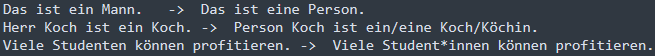
\includegraphics[width=9cm]{Resources/Substitution.PNG}
\caption{Beispielsätze und genderneutraler Substitutionsergebnisse}
\label{fig:substitute}
\end{figure}

% --- Theoretische Betrachtung der Verfügbarmachung
\section{Bereitstellung}
\label{sec:bereitstellung}
%Felix

In der Zielgruppenanalyse wurden mehrere Anforderungen herausgearbeitet, welche die Anwendung erfüllen muss, damit eine hohe Nutzungsrate erreicht wird. Eine einfache Benutzbarkeit, sowie eine einfache, flexible und mobile Verwendung der Applikation sind von Relevanz. Die einfache Benutzbarkeit wird durch eine schlichte und intuitive Bedienoberfläche sichergestellt, während für die flexible und mobile Verwendung die Art der Bereitstellung der Software eine Rolle spielt.

Es wurde beschlossen, dass Equaly als Webanwendung ausgelegt wird. Da ein Browser mit Internetzugriff auf fast jedem netzwerkfähigem Gerät vorhanden ist, können die Nutzer*innen das Tool plattformunabhängig verwenden. Die Anwendung der Software ist dadurch nicht mehr auf ein bestimmtes Betriebssystem oder eine Gerätart beschränkt.

Des Weiteren ist auch der Betrieb des Webservers für die Bereitstellung der Anwendung plattformunabhängig möglich. Das Backend wurde mittels Java 8 implementiert. Java ist für alle gängigen Betriebssysteme verfügbar, sodass auf jedem Rechner, auf dem Java installiert ist, der Webserver für Equaly eingerichtet werden kann. Zusätzliche Frameworks, Bibliotheken und Techniken, die bei der Implementation des Backends zum Einsatz kamen, sind alle innerhalb einer JAR-Datei integriert, sodass die einzige Voraussetzung für die Einrichtung des Servers die Installation von Java 8 ist. \\
Der Quellcode und eine Installationsanleitung werden veröffentlicht, damit Institutionen und Individuen mit Interesse an dem Softwareprojekt sich es runterladen und ohne Probleme ausführen können.

% Bei der Bereitstellung kannst du zusammenfassend kurz darauf eingehen, welche Zielgruppen wir identifiziert haben und wie die bestmöglich erreicht werden können: Mit der entwickelten Web-Anwendung (das sollten maximal 2-3 Sätze sein, weil diese Entscheidung hier ja schon getroffen (und oben schon angesprochen) wurde)
% Du konkretisierst dass dann aber z.B. dahingehend, das die Verwendung von Java uns den Faktor der Plattformunabhängigkeit für den Betrieb des Backends erlaubt hat.
% Dann kannste auch sagen, dass die Kombination aus den verwendeten Frameworks, Bibliotheken und Techniken eine Integration aller Notwendigkeiten in eine einzige JAR-Datei ermöglichte
% Als einzige Voraussetzung braucht man also nur Java 8
% Der Quellcode und eine Installationsanleitung werden veröffentlicht, der Betrieb ist zunächst so gedacht, das Institutionen mit Interesse an diesem Projekt dieses runterladen und dann eben easy laufen lassen können
% --- Theoretische Betrachtung der Qualitätssicherung (Tests, Tag des Beta-Testens) ---
\input{Contents/Qualitätssicherung}
% --- Diskussion (Schlussfolgerungen aus Ergebnissen, Möglichkeiten für zukünftige Arbeiten, indirekt auch Ausblick auf mögliche zukünftige Arbeiten) ---
\begin{figure*}[!t]
    \centering
    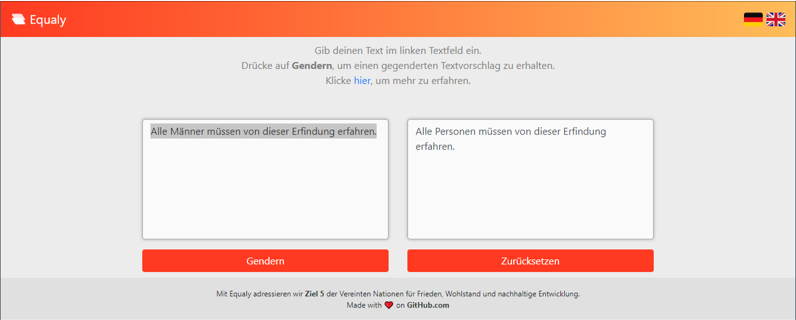
\includegraphics[width=14cm]{Resources/image.png}
    \caption{Realisierte Weboberfläche von Equaly}
    \label{fig:equaly}
\end{figure*}
\section{Diskussion}
\label{sec:diskussion}

Im Rahmen des Moduls ``Software Engineering II'' wurden unterschiedliche Themen behandelt, um den Student*innen die notwendige Theorie näherzubringen, die benötigt wird, um das jeweilige Softwareprojekt unter Durchlauf der Phasen des Software-Engineering realisieren zu können.

Dabei wurden die Vorlesungen des Moduls unter drei unterschiedlichen Professor*innen und Dozent*innen aufgeteilt, wobei jede Person einen anderen Aspekt der Thematik übernommen hat. Anhand der Projektarbeit konnten die Studierenden praktische Erfahrung sammeln, wie der Entwicklungsprozess einer Software aufgebaut ist. Es wurden unter anderem Grundsätze, Entscheidungsschemata und Methodiken für den Entwurf von Bedienoberflächen gelehrt. Außerdem wurde sich innerhalb des Kurses umfassend mit der Implementierung, der Qualitätssicherung und dem Testen, sowie der Dokumentation und der Auslieferung von Software befasst.

Von Anfang an mussten die Student*innen strukturiert an das Projekt herangehen und sich über das gesamte Semester hinweg wie professionelle Entwicklerteams selbstständig organisieren. Diese Selbstständigkeit gepaart mit der Disziplin innerhalb des Projektteams, dem gesammelten Wissen und der gesammelten Erfahrung wird in Zukunft bei möglichen anderen Projekten sehr hilfreich sein.
% Was schreib ich hier?
Anzumerken ist, dass wir (leider) zu Beginn des Projekts die Relevanz unserer Software unterschätzt haben. Equaly hat das Potenzial ein Tool des alltäglichen Gebrauchs zu sein, welches sowohl von Personen der Öffentlichkeit, als auch von Privatpersonen benötigt wird. Falls wir uns dazu entschließen, ein weiteres Softwareprojekt mit einem ähnlichen Ziel zu starten, werden wir in Betracht ziehen, nach offizieller Unterstützung von Sponsoren zu suchen.
% Seriously, was schreib ich hier???
% --- Fazit (Schlussfolgerungen und zukünftige Arbeiten) ---
\section{Fazit}
\label{sec:fazit}
%Marcus

Mit der vorliegenden Arbeit beschreiben wir die Anwendung der Phasen, Techniken und Strategien der Softwareentwicklung anhand eines praktischen Kursprojekts. Die Erarbeitung und Entwicklung fand im Rahmen des Moduls SWE II der HWR Berlin statt. Im Rahmen des Kurses wurde die Entwicklung einer Software zur Adressierung eines der 17 Ziele der United Nations vorgegeben. Das Team entschied sich, Software als Beitrag für die Geschlechtergleichheit zu entwickeln \cite{Un21}. Dazu wurde eine Zielgruppenanalyse durchgeführt. Die erkannten Zielgruppen wurden u.A. mit Gewohnheiten, Arbeitsumfeld und Art der Arbeit als Grundlage für die Architektur der Software, das Design der Oberfläche und die Art der Bereitstellung genutzt. Für diesen gesamten Prozess, sowie für die resultierende Implementierungsarbeit, wird die Arbeitsweise beschrieben. Zentral werden ebenfalls die Maßnahmen der Qualitätssicherung, wie auch ein durchgeführter Beta-Test beleuchtet.

Ergebnis ist die in \ref{fig:equaly} gezeigte Web-Applikation Equaly. Als Ergebnis eines weiterentwickelten Prototyps kann Equaly unter Verwendung von Java und den Frameworks Spring, OpenNLP und Lingua eingegebenen Text aufnehmen, zerlegen, analysieren und zu einem genderneutralen Textvorschlag umformen. Diese Funktionalität wurde für die deutsche und die englische Sprache realisiert. Die Software erfüllt die erwartete Funktionalität. Bestimmte Ungenauigkeiten in der Vorschlagserzeugung mussten zeitbedingt erhalten bleiben. Diese Problemstellungen versprechen eine interessante Grundlage für zukünftige Arbeiten mit NLP-Technologien hin zu einer Anwendung für genderneutrale Textgenerierung zu sein.

% --- Quellen (Bibliography: style and .bib) ---
\bibliographystyle{IEEEtran}
\bibliography{IEEEabrv,bib2SERP13}
% trigger a \newpage just before the given reference
% number - used to balance the columns on the last page
% adjust value as needed - may need to be readjusted if
% the document is modified later
%\IEEEtriggeratref{18}
% The "triggered" command can be changed if desired:
%\IEEEtriggercmd{\enlargethispage{-5in}}


\end{document}


